\documentclass{article}
\usepackage[preprint]{neurips_2023}

\usepackage[utf8]{inputenc} % allow utf-8 input
\usepackage[T1]{fontenc}    % use 8-bit T1 fonts
\usepackage{hyperref}       % hyperlinks
\usepackage{url}            % simple URL typesetting
\usepackage{booktabs}       % professional-quality tables
\usepackage{amsfonts}       % blackboard math symbols
\usepackage{nicefrac}       % compact symbols for 1/2, etc.
\usepackage{microtype}      % microtypography
\usepackage{xcolor}         % colors

\usepackage{amsmath}
\usepackage{graphicx}
\usepackage{algorithm}
\usepackage[noend]{algpseudocode}

\DeclareMathOperator{\softmax}{softmax}
\DeclareMathOperator{\sigmoid}{sigmoid}
\DeclareMathOperator{\sign}{sign}
\DeclareMathOperator{\relu}{ReLU}

\title{Deep Convolutional Neural Networks for Semantic Segmentation}

\author{
  Merrick Qiu\\
  UC San Diego\\
  La Jolla, CA 92093 \\
  \texttt{myqiu@ucsd.edu} \\
  \And
  Michael Ye \\
  UC San Diego \\
  La Jolla, CA 92093 \\
  \texttt{mhye@ucsd.edu} \\
  \AND
  Collin Cranston \\
  UC San Diego \\
  La Jolla, CA 92093 \\
  \texttt{ccransto@ucsd.edu} \\
}



\begin{document}


\maketitle


\begin{abstract}
  We used a deep convolutional neural network in order to perform semantic segmentation on
  the PASCAL VOC 2012 dataset. 
  We built a PyTorch CNN with ReLU activation function, batch normalization, and an encoder and decoder architecture.
  With the baseline model we were able to get a mean pixel accuracy of $83.536\%$ and mean IoU score of $0.24001$ but after 
  weighting classes and applying learning rate scheduling
  we were able to get a model with a mean pixel accuracy of $84.398\%$ and a mean IoU score of $0.25238$.
  While we experimented with a variety of techniques to improve the baseline, only the
  learning rate scheduler and weighted loss ultimately improved our model performance. Data Augmentation failed
  to improve our model, which we attributed to an insuffient number of epochs during training.
\end{abstract}


\section{Introduction}
\subsection{Overview}
Semantic segmentation is the process by which the pixels in an image are classified into a number of categories.
In the PASCAL VOC 2012 dataset, each pixel is classified into one of 21 classes using a softmax.
This is useful in a number of fields including self-driving cars, medical imaging, and satellite imaging.
However, this is a challenging task because it requires the model to understand the context of the image and to be able to
distinguish between different objects. 

To perform semantic segmentation, we used a deep convolutional neural network with an encoder and decoder architecture.
Convolutions can calculate the features of an image by repeatedly applying a filter to an image.
We use ReLU as our acitvation function to add nonlinearity to the network. 
Batch normalization normalizes the input to each layer so that it has zero mean and scaling it to the standard deviation.
This speeds up training and makes the model more robust.
To perform a feedforward pass,
the encoder is used to extract features from the image and the decoder is used to upsample the features to the original image size.


\subsection{Xavier Weight Initialization}
The output from a matrix multiplication has a variance equal to the 
the size of the input vector if the weights and inputs 
are all initated with standard normal distributions.
In addition, the activation function can change the variance of the output.
In order to prevent activations from exploding or vanishing during the forward pass of the initial model,
the weights are set using Xavier weight initialization.

We want the variance of the layer outputs to be 1, which approximately happens when 
the weight values are chosen from the uniform distribution 
$\mathcal{U}(-\sqrt{6/(n_i + n_{i+1})}, \sqrt{6/(n_i + n_{i+1})})$,
where $n_i$ is the fan-in and $n_{i+1}$ is the fan-out.
This distribution comes from research done by Glorot and Bengio (2010) \cite{Xavier_2010}.

\section{Related Work}
The steps used in the model are inspired by techniques found by previous researchers.
Convolutional neural networks were popularized by the paper by Yann LeCun et al. (1989) \cite{LeCun_1989} on handwritten zip code recognition.
As already stated, Xavier weight initialization is used as defined in the paper by Glorot and Bengio (2010) \cite{Xavier_2010}.
Batch normalization was first proposed by Sergey Ioffe and Christian Szegedy (2015)\cite{Ioffe_2015}.
Finally, the use of a convolutional neural network for image segmentation 
has also been done by Olaf Ronneberger et al. (2015) with their U-Net architecture \cite{Ronneberger_2015}
and by Kaiming He et al. (2018) \cite{Kaiming_2018} with their Mask R-CNN architecture.


\section{Methods}
\subsection{Basline Model architecture}

The architecture of the basline model is shown in table 1.
\begin{table}[h!]
\caption{Baseline model architecture}
\label{tab:baseline_model_architecture}
\centering
\begin{tabular}{cccc}
  \toprule
  \textbf{Type} & \textbf{Output Channels} & \textbf{Kernel Size / Stride / Padding} & \textbf{Activation Function} \\ 
  \midrule
  Conv2d & 32 & 3x3 / 2 / 1 & ReLU \\ 
  BatchNorm2d & 32 & - & - \\ 
  Conv2d & 64 & 3x3 / 2 / 1 & ReLU \\ 
  BatchNorm2d & 64 & - & - \\ 
  Conv2d & 128 & 3x3 / 2 / 1 & ReLU \\ 
  BatchNorm2d & 128 & - & - \\ 
  Conv2d & 256 & 3x3 / 2 / 1 & ReLU \\ 
  BatchNorm2d & 256 & - & - \\ 
  Conv2d & 512 & 3x3 / 2 / 1 & ReLU \\ 
  BatchNorm2d & 512 & - & - \\ 
  ConvTranspose2d & 512 & 3x3 / 2 / 1 / 1 & ReLU \\ 
  BatchNorm2d & 512 & - & - \\ 
  ConvTranspose2d & 256 & 3x3 / 2 / 1 / 1 & ReLU \\ 
  BatchNorm2d & 256 & - & - \\ 
  ConvTranspose2d & 128 & 3x3 / 2 / 1 / 1 & ReLU \\ 
  BatchNorm2d & 128 & - & - \\ 
  ConvTranspose2d & 64 & 3x3 / 2 / 1 / 1 & ReLU \\ 
  BatchNorm2d & 64 & - & - \\ 
  ConvTranspose2d & 32 & 3x3 / 2 / 1 / 1 & ReLU \\ 
  BatchNorm2d & 32 & - & - \\ 
  Conv2d(Classifier) & n\_class & 1x1 / - / - & - \\ 
  \bottomrule
\end{tabular}
\end{table}

\subsection{Experimental Architecture}
\subsubsection{Experimental Architecture I}
The following experimental architecture tries to integrate fully connected layers into the model.
However, the model did not perform as well as the baseline model and took much longer to train due to the extra weights.
The model early stopped at around 7 epochs and is only able to obtain an accuracy of $0.75$ and IoU of $0.056$.
\begin{table}[h!]
\caption{Experimental architecture 1}
\label{tab:experimental_1}
\centering
\begin{tabular}{cccc}
  \toprule
  \textbf{Type} & \textbf{Output Channels} & \textbf{Kernel Size / Stride / Padding} & \textbf{Activation Function} \\ 
  \midrule
  Conv2d & 64 & 3x3 / 1 / 1 & ReLU \\ 
  BatchNorm2d & 64 & - & - \\ 
  Conv2d(Fully Connected) & 64 & 1x1 / 1 / 1 & - \\
  Conv2d & 64 & 3x3 / 1 / 1 & ReLU \\ 
  BatchNorm2d & 64 & - & - \\ 
  Conv2d(Fully Connected) & 64 & 1x1 / 1 / 1 & - \\
  Conv2d & 64 & 3x3 / 1 / 1 & ReLU \\ 
  BatchNorm2d & 64 & - & - \\ 
  Conv2d(Fully Connected) & 64 & 1x1 / 1 / 1 & - \\
  Conv2d & 64 & 3x3 / 1 / 1 & ReLU \\ 
  BatchNorm2d & 64 & - & - \\ 
  Conv2d(Fully Connected) & 64 & 1x1 / 1 / 1 & - \\
  Conv2d & 64 & 3x3 / 1 / 1 & ReLU \\ 
  BatchNorm2d & 64 & - & - \\ 
  Conv2d(Classifier) & n\_class & 1x1 / - / - & - \\ 
  \bottomrule
\end{tabular}
\end{table}
\subsubsection{Experimental Architecture II}
The following experimental architecture is the ResNet-50 model in the PyTorch Library.
This model introduces a new term - Cfg Blocks, which are comprised of $1$ Conv layer
with multiple Identity layers. Cfg0 contains 1 Conv Layer with 2 Identity layers
and has a $(56, 56, 64)$ input shape and $(56, 56, 256)$ output shape.
Cfg1 contains 1 Conv layer with 2 Identity layers again, this time with a 
$(56, 56, 256)$ input shape and $(28, 28, 512)$ output shape.
Cfg2 Block has 1 conv layer and 5 Identity layers with a $(28, 28, 512)$ input shape and
a $(14, 14, 1024)$ output shape. Lastly, Cfg3 block contains 1 Conv Layer and 2 Identity layers
with an input shape of $(14, 14, 1024)$ and an output shape of $(7, 7, 2048)$. The entire
architecture is displayed below.
\begin{table}[h!]
  \caption{Experimental architecture II}
  \label{tab:experimental_2}
  \centering
  \begin{tabular}{ccc}
    \toprule
    \textbf{Type} & \textbf{Output Shape} & Parameters \\ 
    \midrule
    input & [(None, 224, 224, 3)] & 0  \\ 
    sequential & (None, 224, 224, 3) & 0 \\ 
    conv2d\_28 & 64 & 9472\\
    max\_pooling2d & 64 & 0 \\ 
    cfg0\_block & 64 & 148480\\ 
    cfg1\_block & 64 & 665600 \\
    cfg2\_block & 64 & 2641920 \\ 
    cfg3\_block & 64 & 10526720  \\ 
    classifier & 64 & 3932280  \\
    \bottomrule
  \end{tabular}
\end{table}


\subsubsection{Experimental Architecture III}

We implemented the U-Net convolutional neural network \cite{unet}, and trained it on the VOC semantic segmentation task. See Table \ref{tab:experimental_3} for the architecture of the model. \\
Without class weights, the U-Net model quickly achieved $75\% $ pixel accuracy, which means the model was simply predicting the background class. To counter this, we implemented class weights, to account for class imbalance and penalize the background labels with lower weights. Despite the validation error steadily decreasing across epochs, the model still experienced spikes in training error. Therefore, we also implemented the cosine annealing learning rate scheduler, and the following data augmentations: random crop, flip, and rotation. 
\begin{table}[H]
\caption{UNet Architecture}
\label{tab:experimental_3}
\centering
\begin{tabular}{cccc}
  \toprule
  \textbf{Type} & \textbf{Input/Output Channels} & \textbf{Kernel Size / Stride / Padding} & \textbf{Activation Function} \\ 
  \midrule
  \textbf{ConvBlock} & in/out & - & - \\
  \hline
  Conv2D & in/out & 3/1/1 & ReLU \\ 
  BatchNorm2d & - & - & - \\ 
  Conv2D & out/out & 3/1/1 & ReLU \\ 
  BatchNorm2d & - & - & - \\ 
  \hline
  \textbf{DownBlock} & in/out & - & - \\
  \hline
  ConvBlock & in/out & - & - \\ 
  MaxPool2d & out/out & - & - \\ 
  \hline
  \textbf{UpBlock} & in/out & - & - \\
  \hline
  ConvTranspose2d& in/in/2 & - & - \\ 
  torch.cat & - & in/2 / in & - \\ 
  ConvBlock & in / out & - & - \\ 
  \hline
  \textbf{UNet} & 3/ n\_classes & - & - \\ 
  \hline
  ConvBlock & 3 /64 & - & - \\
  DownBlock & 64 / 128 & - & - \\
  DownBlock & 128 /256 & - & - \\
  DownBlock & 256 /512 & - & - \\
  DownBlock & 512/ 1024 & - & - \\
  ConvBlock & 1024 /1024 & - & - \\
  UpBlock & 1024/ 512 & - & - \\
  UpBlock & 512 /256 & - & - \\
  UpBlock & 256 /128 & - & - \\
  UpBlock & 128/ 64 & - & - \\
  Conv2d & 64 /n\_classes & - & - \\
  \bottomrule
\end{tabular}
\end{table}


\section{Results}
\subsection{Model Metrics}

\begin{table}[H]
  \caption{IOU and Pixel Accuracy Metrics}
  \centering
  \begin{tabular}{lll}
    \toprule
    \cmidrule(r){1-2}
    Model & IOU & Pixel Accuracy   \\
    \midrule
    Baseline                   & $0.24001$ & $83.536\%$  \\
    Learning Rate Scheduling   & $0.25927$ & $83.954\%$  \\
    Data Augmentation          & $0.10226$ & $77.803\%$  \\
    Weighted Classes           & $0.25238$ & $84.398\%$  \\
    \bottomrule
  \end{tabular}
\end{table}
\subsection{Loss Graphs}
\begin{figure}[H]
  \centering
  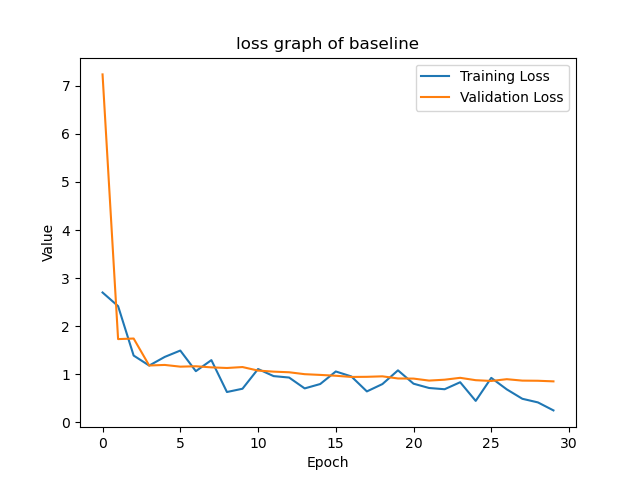
\includegraphics[width=6cm]{baseline.png}
  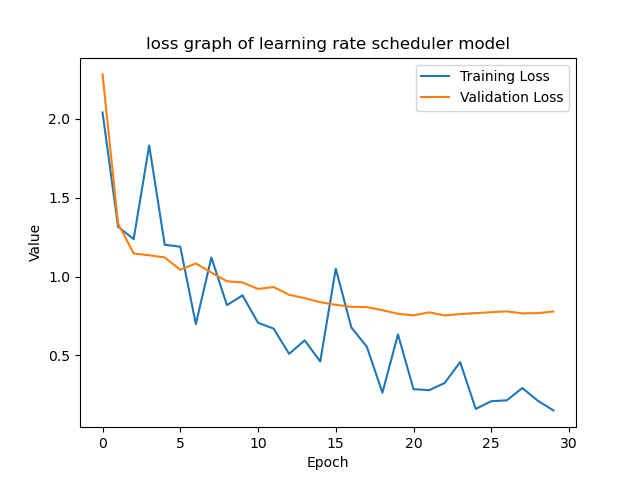
\includegraphics[width=6cm]{learning rate scheduler model.png}
  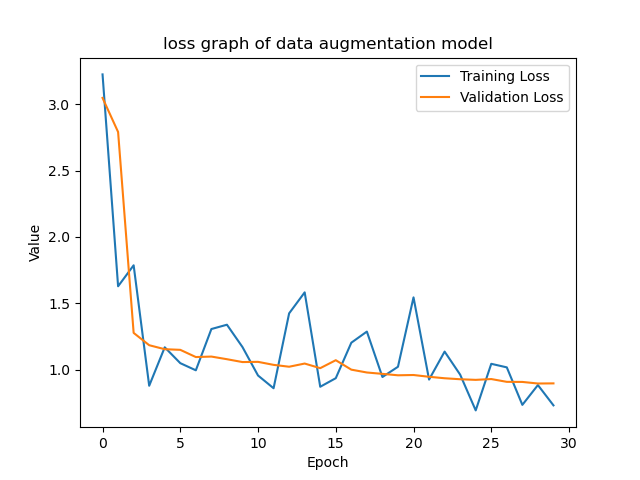
\includegraphics[width=6cm]{data augmentation model.png}
  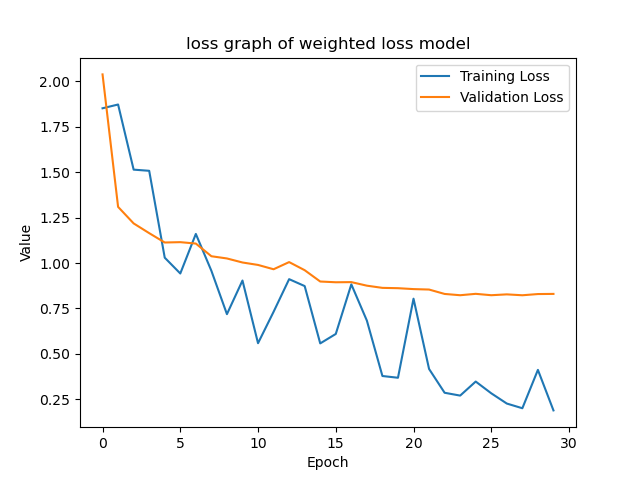
\includegraphics[width=6cm]{weighted loss model.png}
  \caption{Training and Validation Loss of Basline, Scheduling, Data Augmentation, and Weighted Class Models}
\end{figure}

\subsection{Output Visualizations}
To visualize our output, we show the output masks of each model 
for a random image from the test set.
\begin{figure}[H]
  \centering
  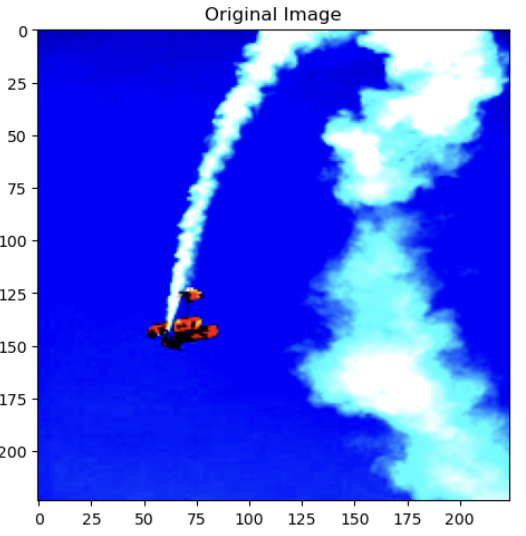
\includegraphics[width=6cm]{Original Image.png}
  \caption{Original Random Test Set Image}
\end{figure}
\begin{figure}[H]
  \centering
  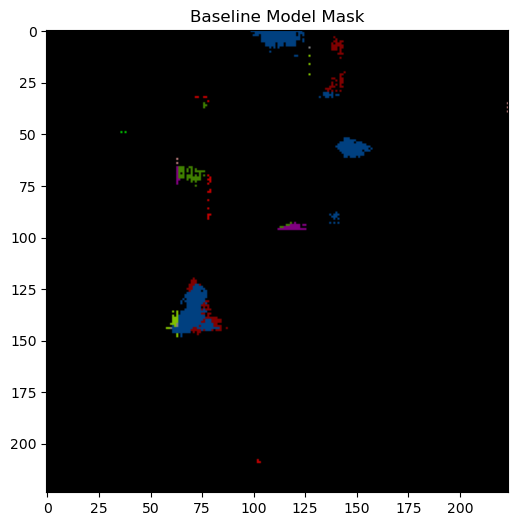
\includegraphics[width=6cm]{baseline visualization.png}
  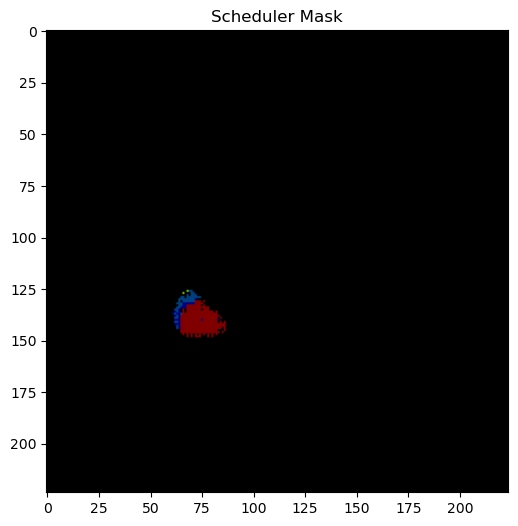
\includegraphics[width=6cm]{scheduler visualization.png}
  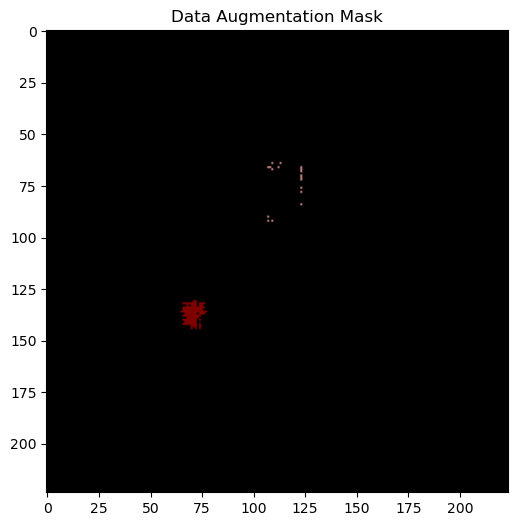
\includegraphics[width=6cm]{data augment visualization.png}
  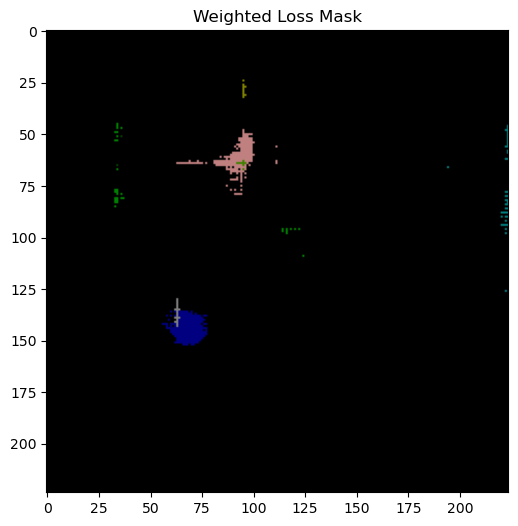
\includegraphics[width=6cm]{weighted loss visualization.png}
  \caption{Output Mask of Basline, Scheduling, Data Augmentation, and Weighted Class Models}
\end{figure}


\section{Discussion}
\subsection{Baseline Model}


\subsection{Improving Baseline Model}
\subsubsection{Cosine Annealing}
\label{cosine}
\subsubsection{Data Augmentation}
\subsubsection{Class Weights}
Due to heavy class imbalances, the baseline model achieved relatively high pixel accuracy $(\sim 83.5 \% )$ while having a low IOU score. The model would predict the most common label (background pixel). In order to counter the class label imbalance, we implemented a power class weight function, which penalizes higher frequency labels with lower weights. \\

In particular, we computed class frequencies ($\text{class}\_\text{freq}$) by counting the number of class instances in each mask, and dividing by the total number of pixels in the mask. To penalize the most frequent labels, we then inverted $\text{class}\_\text{freq}$
\begin{equation}
    \text{class}\_\text{weight}=1.0 / \text{class}\_\text{freq}
\end{equation}
and normalized to sum to the number of classes, 21, 
\begin{equation}
    \text{class}\_\text{weight}=\text{class}\_\text{weight} / \text{sum}(\text{class}\_\text{weight}) * \text{num}\_\text{classes}
\end{equation}

After implementing class weights, the model experienced a slight improvement over the baseline model, both in pixel accuracy and IOU. Weighted classes is a useful tool to combat class imbalance, particularly in semantic segmentation where some pixels (e.g background) can heavily dominate in training labels.


\subsection{Experimentation}
See Table 5 for metrics for all experimental models:

\begin{table}[H]
  \caption{IOU and Pixel Accuracy Metrics}
  \centering
  \begin{tabular}{lll}
    \toprule
    \cmidrule(r){1-2}
    Model & IOU & Pixel Accuracy   \\
    \midrule
    Baseline                   & $0.24000997841358185$ & $0.835359513759613$  \\
    Alternate   & $0.056$ & $0.75$  \\
    Pre-trained ResNet          & $0.40788033604621887$ & $0.9090900421142578$  \\
    U-Net           & $0.10018574446439743$ & $0.6077122688293457 $  \\
    \bottomrule
  \end{tabular}
\end{table}

\subsubsection{Alternate Model}

\subsubsection{Transfer Learning}

\subsubsection{U-Net Model}
We implemented the U-Net architecture from \cite{unet}, which is a form of a Convolutional Neural Network (\textbf{CNN}) that involves the use of skip connections, and encoding/decoder blocks. Due to the more complex architecture, U-Net's took longer to train. Moreover, our U-Net experienced pathological training behavior, with training spikes in later epochs ($20+$). \\
In order to combat the loss spikes during training, we applied several techniques. First, we tuned hyperparameters such as the learning rate, and early stopping mechanism. Next, we applied cosine annealing from \ref{cosine}, and also clipped gradients to avoid spikes in loss. Moreover, we used class weights, as the U-net experienced similar issues as the baseline model with learning to predicting the background class. Without class weights, the U-Net model would quickly jump to $\sim 75\%$ pixel accuracy, and remain stagnant throughout training. \\
Despite being originally developed for biological image segmentation, the U-Net performed worse than both the ResNet and baseline model on our VOC dataset segmentation task. While the training graph (Fig \ref{fig:2} ) shows steady improvement over 30 epochs, the training loss spikes indicate a need for finer tuning of the model. 

\begin{figure}[H]
    \centering
    
\includegraphics[width=0.5\linewidth]{Report/Unet final.png}
    \caption{U-Net Training Dynamics}
    \label{fig:2}
\end{figure}

%will do-collin

\newpage
\section*{Authors' Contributions}
\textbf{Merrick:} I implemented the evaluation metrics, baseline model
(including the train(), val(), modelTest() functions for the baseline model), early stopping, and
helped debug with data augmentation.
I also created the experimental architecture for part (a) of Experimentation and your solution.
I helped write the report, especially the 
abstract, introduction, related work, and references sections.

\textbf{Michael:} I implemented the learning rate scheduler, data augmentation, train and validation 
loss plotting functions, transfer learning models, and data visualization. Additionally I made improvements
to the model's efficiency by tuning the $num\_workers$ variable
to increase training speed. I wrote the results section and part of the methodology section
of the report.

\textbf{Collin:}
I implemented the U-Net model in the experimental section (5c). I also implemented the data loading for test and 
validation sets (voc.py), weighted class function, and helped create plots and debug. I also helped write the report, 
especially the methods and discussion sections.

\bibliographystyle{plain} 
\bibliography{refs}
\end{document}
